% Options for packages loaded elsewhere
\PassOptionsToPackage{unicode}{hyperref}
\PassOptionsToPackage{hyphens}{url}
\PassOptionsToPackage{dvipsnames,svgnames,x11names}{xcolor}
%
\documentclass[
  a4paper,
  DIV=11,
  numbers=noendperiod]{scrartcl}

\usepackage{amsmath,amssymb}
\usepackage{iftex}
\ifPDFTeX
  \usepackage[T1]{fontenc}
  \usepackage[utf8]{inputenc}
  \usepackage{textcomp} % provide euro and other symbols
\else % if luatex or xetex
  \usepackage{unicode-math}
  \defaultfontfeatures{Scale=MatchLowercase}
  \defaultfontfeatures[\rmfamily]{Ligatures=TeX,Scale=1}
\fi
\usepackage{lmodern}
\ifPDFTeX\else  
    % xetex/luatex font selection
  \setmainfont[]{Spectral}
  \setsansfont[]{Roboto}
  \setmonofont[]{JetBrainsMono-Regular}
\fi
% Use upquote if available, for straight quotes in verbatim environments
\IfFileExists{upquote.sty}{\usepackage{upquote}}{}
\IfFileExists{microtype.sty}{% use microtype if available
  \usepackage[]{microtype}
  \UseMicrotypeSet[protrusion]{basicmath} % disable protrusion for tt fonts
}{}
\makeatletter
\@ifundefined{KOMAClassName}{% if non-KOMA class
  \IfFileExists{parskip.sty}{%
    \usepackage{parskip}
  }{% else
    \setlength{\parindent}{0pt}
    \setlength{\parskip}{6pt plus 2pt minus 1pt}}
}{% if KOMA class
  \KOMAoptions{parskip=half}}
\makeatother
\usepackage{xcolor}
\usepackage[top=25mm,left=40mm,right=30mm,bottom=25mm,heightrounded]{geometry}
\setlength{\emergencystretch}{3em} % prevent overfull lines
\setcounter{secnumdepth}{-\maxdimen} % remove section numbering
% Make \paragraph and \subparagraph free-standing
\ifx\paragraph\undefined\else
  \let\oldparagraph\paragraph
  \renewcommand{\paragraph}[1]{\oldparagraph{#1}\mbox{}}
\fi
\ifx\subparagraph\undefined\else
  \let\oldsubparagraph\subparagraph
  \renewcommand{\subparagraph}[1]{\oldsubparagraph{#1}\mbox{}}
\fi


\providecommand{\tightlist}{%
  \setlength{\itemsep}{0pt}\setlength{\parskip}{0pt}}\usepackage{longtable,booktabs,array}
\usepackage{calc} % for calculating minipage widths
% Correct order of tables after \paragraph or \subparagraph
\usepackage{etoolbox}
\makeatletter
\patchcmd\longtable{\par}{\if@noskipsec\mbox{}\fi\par}{}{}
\makeatother
% Allow footnotes in longtable head/foot
\IfFileExists{footnotehyper.sty}{\usepackage{footnotehyper}}{\usepackage{footnote}}
\makesavenoteenv{longtable}
\usepackage{graphicx}
\makeatletter
\def\maxwidth{\ifdim\Gin@nat@width>\linewidth\linewidth\else\Gin@nat@width\fi}
\def\maxheight{\ifdim\Gin@nat@height>\textheight\textheight\else\Gin@nat@height\fi}
\makeatother
% Scale images if necessary, so that they will not overflow the page
% margins by default, and it is still possible to overwrite the defaults
% using explicit options in \includegraphics[width, height, ...]{}
\setkeys{Gin}{width=\maxwidth,height=\maxheight,keepaspectratio}
% Set default figure placement to htbp
\makeatletter
\def\fps@figure{htbp}
\makeatother
\newlength{\cslhangindent}
\setlength{\cslhangindent}{1.5em}
\newlength{\csllabelwidth}
\setlength{\csllabelwidth}{3em}
\newlength{\cslentryspacingunit} % times entry-spacing
\setlength{\cslentryspacingunit}{\parskip}
\newenvironment{CSLReferences}[2] % #1 hanging-ident, #2 entry spacing
 {% don't indent paragraphs
  \setlength{\parindent}{0pt}
  % turn on hanging indent if param 1 is 1
  \ifodd #1
  \let\oldpar\par
  \def\par{\hangindent=\cslhangindent\oldpar}
  \fi
  % set entry spacing
  \setlength{\parskip}{#2\cslentryspacingunit}
 }%
 {}
\usepackage{calc}
\newcommand{\CSLBlock}[1]{#1\hfill\break}
\newcommand{\CSLLeftMargin}[1]{\parbox[t]{\csllabelwidth}{#1}}
\newcommand{\CSLRightInline}[1]{\parbox[t]{\linewidth - \csllabelwidth}{#1}\break}
\newcommand{\CSLIndent}[1]{\hspace{\cslhangindent}#1}

\addtokomafont{disposition}{\rmfamily}
\KOMAoption{captions}{tableheading}
\makeatletter
\makeatother
\makeatletter
\makeatother
\makeatletter
\@ifpackageloaded{caption}{}{\usepackage{caption}}
\AtBeginDocument{%
\ifdefined\contentsname
  \renewcommand*\contentsname{Table of contents}
\else
  \newcommand\contentsname{Table of contents}
\fi
\ifdefined\listfigurename
  \renewcommand*\listfigurename{List of Figures}
\else
  \newcommand\listfigurename{List of Figures}
\fi
\ifdefined\listtablename
  \renewcommand*\listtablename{List of Tables}
\else
  \newcommand\listtablename{List of Tables}
\fi
\ifdefined\figurename
  \renewcommand*\figurename{Figure}
\else
  \newcommand\figurename{Figure}
\fi
\ifdefined\tablename
  \renewcommand*\tablename{Table}
\else
  \newcommand\tablename{Table}
\fi
}
\@ifpackageloaded{float}{}{\usepackage{float}}
\floatstyle{ruled}
\@ifundefined{c@chapter}{\newfloat{codelisting}{h}{lop}}{\newfloat{codelisting}{h}{lop}[chapter]}
\floatname{codelisting}{Listing}
\newcommand*\listoflistings{\listof{codelisting}{List of Listings}}
\makeatother
\makeatletter
\@ifpackageloaded{caption}{}{\usepackage{caption}}
\@ifpackageloaded{subcaption}{}{\usepackage{subcaption}}
\makeatother
\makeatletter
\@ifpackageloaded{tcolorbox}{}{\usepackage[skins,breakable]{tcolorbox}}
\makeatother
\makeatletter
\@ifundefined{shadecolor}{\definecolor{shadecolor}{rgb}{.97, .97, .97}}
\makeatother
\makeatletter
\makeatother
\makeatletter
\makeatother
\ifLuaTeX
  \usepackage{selnolig}  % disable illegal ligatures
\fi
\IfFileExists{bookmark.sty}{\usepackage{bookmark}}{\usepackage{hyperref}}
\IfFileExists{xurl.sty}{\usepackage{xurl}}{} % add URL line breaks if available
\urlstyle{same} % disable monospaced font for URLs
\hypersetup{
  pdftitle={Group Name's Group Project},
  colorlinks=true,
  linkcolor={blue},
  filecolor={Maroon},
  citecolor={Blue},
  urlcolor={Blue},
  pdfcreator={LaTeX via pandoc}}

\title{Group Name's Group Project}
\author{}
\date{}

\begin{document}
\maketitle
\ifdefined\Shaded\renewenvironment{Shaded}{\begin{tcolorbox}[frame hidden, interior hidden, borderline west={3pt}{0pt}{shadecolor}, boxrule=0pt, enhanced, breakable, sharp corners]}{\end{tcolorbox}}\fi

\hypertarget{declaration-of-authorship}{%
\subsection*{Declaration of
Authorship}\label{declaration-of-authorship}}

We, {[}DeskB{]}, confirm that the work presented in this assessment is
our own. Where information has been derived from other sources, we
confirm that this has been indicated in the work. Where a Large Language
Model such as ChatGPT has been used we confirm that we have made its
contribution to the final submission clear.

Date: December 11th 2023

Student Numbers: 20017359 23032922 23081403 23103585 23130397

\hypertarget{brief-group-reflection}{%
\subsection{Brief Group Reflection}\label{brief-group-reflection}}

\begin{longtable}[]{@{}ll@{}}
\toprule\noalign{}
What Went Well & What Was Challenging \\
\midrule\noalign{}
\endhead
\bottomrule\noalign{}
\endlastfoot
A & B \\
C & D \\
\end{longtable}

\hypertarget{priorities-for-feedback}{%
\subsection{Priorities for Feedback}\label{priorities-for-feedback}}

Are there any areas on which you would appreciate more detailed feedback
if we're able to offer it?

\newpage{}

\hypertarget{response-to-questions}{%
\section{Response to Questions}\label{response-to-questions}}

\hypertarget{who-collected-the-data}{%
\subsection{1. Who collected the data?}\label{who-collected-the-data}}

1.\href{http://data.insideairbnb.com/united-kingdom/england/london/2023-09-06/data/listings.csv.gz}{*listings.csv}
: This dataset was created by automatically scraping public information
from Airbnb's Website. Murray Cox was one of the main founder and
technicians of this mission driven project that aims to provide data and
advocacy about Airbnb's impact on residential communities.
\href{(http://insideairbnb.com/about)}{{[}1{]}}
2.\href{https://data.london.gov.uk/download/london_boroughs/9502cdec-5df0-46e3-8aa1-2b5c5233a31f/London_Boroughs.gpkg}{*London\_Boroughs.gpkg}
and
\href{https://data.london.gov.uk/download/statistical-gis-boundary-files-london/08d31995-dd27-423c-a987-57fe8e952990/London-wards-2018.zip}{London-wards-2018}
: This dataset is an extract from
\href{https://www.ordnancesurvey.co.uk/}{Ordnance Survey} Boundary-Line
product which is a specialist 1:10 000 scale boundaries dataset.

( 2 points; Answer due Week 7 )

An inline citation: As discussed on {`Inside airbnb'} (n.d.), there are
many\ldots{}

A parenthetical citation: There are many ways to research Airbnb (see,
for example, {`Inside airbnb'}, n.d.)\ldots{}

\hypertarget{why-did-they-collect-it}{%
\subsection{2. Why did they collect it?}\label{why-did-they-collect-it}}

( 4 points; Answer due Week 7 )
1.\href{http://data.insideairbnb.com/united-kingdom/england/london/2023-09-06/data/listings.csv.gz}{*listings.csv}
: Inside Airbnb is a mission driven project that provides data and
advocacy about Airbnb's impact on residential communities. We work
towards a vision where communities are empowered with data and
information to understand, decide and control the role of renting
residential homes to tourists.
2.\href{https://data.london.gov.uk/download/london_boroughs/9502cdec-5df0-46e3-8aa1-2b5c5233a31f/London_Boroughs.gpkg}{*London\_Boroughs.gpkg}
: With a long history and evolving from . The Ordnance Survey aims to
help governments make smarter decisions that ensure our safety and
security, they also show businesses how to gain a location data edge and
we help everyone experience the benefits of the world outside.

\begin{verbatim}
Data frame is 69,351 x 76
\end{verbatim}

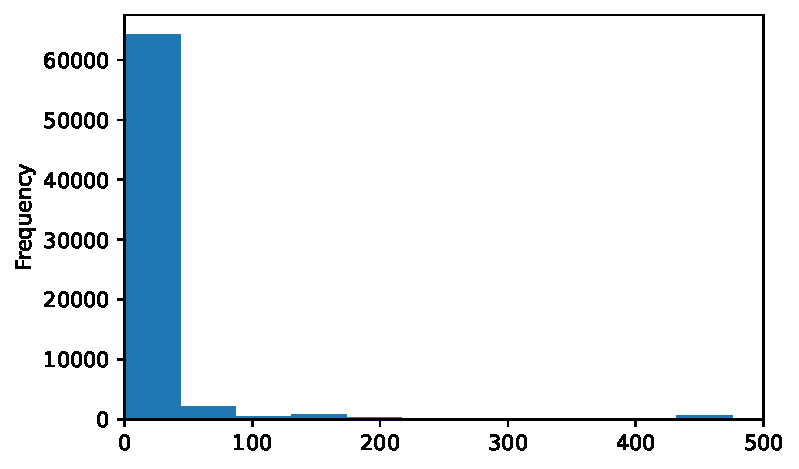
\includegraphics{Group_Work_DeskB_files/figure-pdf/cell-5-output-1.pdf}

\hypertarget{how-was-the-data-collected}{%
\subsection{3. How was the data
collected?}\label{how-was-the-data-collected}}

1.\href{http://data.insideairbnb.com/united-kingdom/england/london/2023-09-06/data/listings.csv.gz}{*listings.csv}
: Inside Airbnb collects its data primarily by scraping information from
the Airbnb website. This process involves the following steps: 1.Web
Scraping: Inside Airbnb uses automated scripts to systematically browse
and extract data from Airbnb's listings. These scripts navigate the
website just like a human user would, but they do it much faster and on
a larger scale. 2.Data Extraction: Information about each listing, such
as location, price, availability, number of bedrooms, reviews, and host
details, is extracted and compiled. 3.Data Aggregation: The collected
data is then aggregated into a database. This database is organized to
make it easier to analyze trends, patterns, and insights related to
Airbnb's offerings in various cities and regions. 4.Regular Updates: The
scraping process is repeated periodically to keep the database current,
capturing new listings and updates to existing ones. 5.Public
Accessibility: The aggregated data is often made available to the public
through the Inside Airbnb website, enabling researchers, policymakers,
and the general public to analyze Airbnb's impact on housing markets and
communities. It's important to note that web scraping practices, like
those used by Inside Airbnb, may face legal and ethical considerations
depending on the website's terms of service and regional laws regarding
data privacy and usage.
2.\href{https://data.london.gov.uk/download/london_boroughs/9502cdec-5df0-46e3-8aa1-2b5c5233a31f/London_Boroughs.gpkg}{*London\_Boroughs.gpkg}
: .

( 5 points; Answer due Week 8 )

\hypertarget{how-does-the-method-of-collection-impact-the-completeness-andor-accuracy-of-its-representation-of-the-process-it-seeks-to-study-and-what-wider-issues-does-this-raise}{%
\subsection{4. How does the method of collection impact the completeness
and/or accuracy of its representation of the process it seeks to study,
and what wider issues does this
raise?}\label{how-does-the-method-of-collection-impact-the-completeness-andor-accuracy-of-its-representation-of-the-process-it-seeks-to-study-and-what-wider-issues-does-this-raise}}

( 11 points; Answer due Week 9 )

\hypertarget{what-ethical-considerations-does-the-use-of-this-data-raise}{%
\subsection{5. What ethical considerations does the use of this data
raise?}\label{what-ethical-considerations-does-the-use-of-this-data-raise}}

( 18 points; Answer due \textbf{?var:assess.group-date} )

\hypertarget{with-reference-to-the-data-i.e.-using-numbers-figures-maps-and-descriptive-statistics-what-does-an-analysis-of-hosts-and-listing-types-suggest-about-the-nature-of-airbnb-lets-in-london}{%
\subsection{\texorpdfstring{6. With reference to the data (\emph{i.e.}
using numbers, figures, maps, and descriptive statistics), what does an
analysis of Hosts and Listing types suggest about the nature of Airbnb
lets in
London?}{6. With reference to the data (i.e. using numbers, figures, maps, and descriptive statistics), what does an analysis of Hosts and Listing types suggest about the nature of Airbnb lets in London?}}\label{with-reference-to-the-data-i.e.-using-numbers-figures-maps-and-descriptive-statistics-what-does-an-analysis-of-hosts-and-listing-types-suggest-about-the-nature-of-airbnb-lets-in-london}}

( 15 points; Answer due \textbf{?var:assess.group-date} )

\hypertarget{drawing-on-your-previous-answers-and-supporting-your-response-with-evidence-e.g.-figures-maps-and-statistical-analysismodels-how-could-this-data-set-be-used-to-inform-the-regulation-of-short-term-lets-stl-in-london}{%
\subsection{\texorpdfstring{7. Drawing on your previous answers, and
supporting your response with evidence (e.g.~figures, maps, and
statistical analysis/models), how \emph{could} this data set be used to
inform the regulation of Short-Term Lets (STL) in
London?}{7. Drawing on your previous answers, and supporting your response with evidence (e.g.~figures, maps, and statistical analysis/models), how could this data set be used to inform the regulation of Short-Term Lets (STL) in London?}}\label{drawing-on-your-previous-answers-and-supporting-your-response-with-evidence-e.g.-figures-maps-and-statistical-analysismodels-how-could-this-data-set-be-used-to-inform-the-regulation-of-short-term-lets-stl-in-london}}

( 45 points; Answer due \textbf{?var:assess.group-date} )

\hypertarget{sustainable-authorship-tools}{%
\subsection{Sustainable Authorship
Tools}\label{sustainable-authorship-tools}}

Your QMD file should automatically download your BibTeX file. We will
then re-run the QMD file to generate the output successfully.

Written in Markdown and generated from
\href{https://quarto.org/}{Quarto}. Fonts used:
\href{https://fonts.google.com/specimen/Spectral}{Spectral} (mainfont),
\href{https://fonts.google.com/specimen/Roboto}{Roboto} ({sansfont}) and
\href{https://fonts.google.com/specimen/JetBrains\%20Mono}{JetBrains
Mono} (\texttt{monofont}).

\hypertarget{references}{%
\subsection*{References}\label{references}}
\addcontentsline{toc}{subsection}{References}

\hypertarget{refs}{}
\begin{CSLReferences}{0}{0}
\leavevmode\vadjust pre{\hypertarget{ref-insideairbnb}{}}%
{`Inside airbnb'} (n.d.). Available at: \url{http://insideairbnb.com}.

\end{CSLReferences}



\end{document}
